\chapter{Example Setup and Run Commands}
\label{app:examplecommands}
The following screenshots show the Docker commands used to create the Docker environment and run the \gls{rails} Docker containers.
\section{Docker in a Windows Environment}
\label{sec:win-cmds}
Docker on Windows 11 relies on a component called \gls{wsl 2} to provide a Linux-like environment for running Docker containers. Docker Desktop installer provides two options:
\begin{itemize}
    \item Use \gls{wsl 2} backend: This is the recommended approach for most users. It leverages \gls{wsl 2} to create a Linux environment for Docker to run containers.
    \item Use Hyper-V backend: This is an alternative that uses Hyper-V virtualization technology. However, \gls{wsl 2} is generally considered more performant and resource-efficient.   
\end{itemize}
This setup is based on using \gls{wsl 2} as it:
\begin{itemize}
    \item offers better performance for running Linux containers compared to Hyper-V.
    \item provides a more native Linux experience for Docker, ensuring compatibility with most Linux container images.
    \item uses the Windows kernel directly, leading to more efficient resource usage.
\end{itemize}
During Docker Desktop installation with the \gls{wsl 2} backend, Docker will automatically configure and set up \gls{wsl 2} if it's not already installed. It will also create a default Linux distribution (usually Ubuntu) within \gls{wsl 2}. Once \gls{wsl 2} is set up, Docker Desktop installs the Docker daemon within the \gls{wsl 2} environment. This daemon is the core process that manages Docker containers.
Docker Desktop provides a Docker \gls{cli} for Windows. This \gls{cli} interacts with the Docker daemon running in the \gls{wsl 2} environment through a remote API. So, when you run Docker commands on Windows, they are translated and sent to the Docker daemon in \gls{wsl 2} for execution.\vspace{5mm} \\
In essence, Docker on Windows 11 leverages \gls{wsl 2} to create a Linux-like environment for running Docker containers. This approach provides a powerful and performant solution for containerization on Windows, while still offering a familiar Windows experience for interacting with Docker.
\begin{figure}[H]
    \centering
    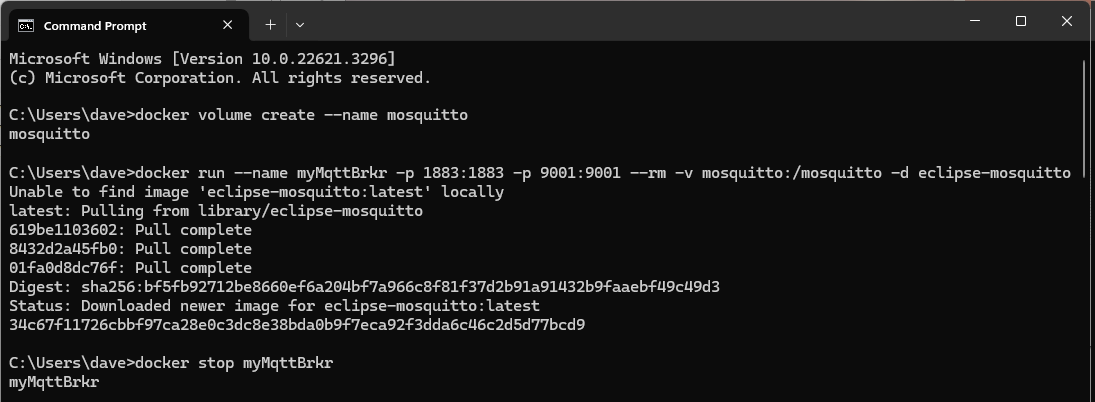
\includegraphics[scale=0.5]{../Images/mosquitto-volume-win.png}
    \caption{Windows Docker mosquitto Setup}
    \label{fig:init-docker-cmds}
\end{figure}
Docker Desktop with \gls{wsl 2} backend stores Docker images and volumes on the Windows file system, accessible from both Windows and \gls{wsl 2}. This allows for easy sharing of container data between the two environments. However, it simpler to use Docker Desktop \gls{gui} to locate and edit the mosquitto configuration file. Figure \ref{fig:volumes-ms} shows the volumes created in the Windows evironment.
\begin{figure}[H]
    \centering
    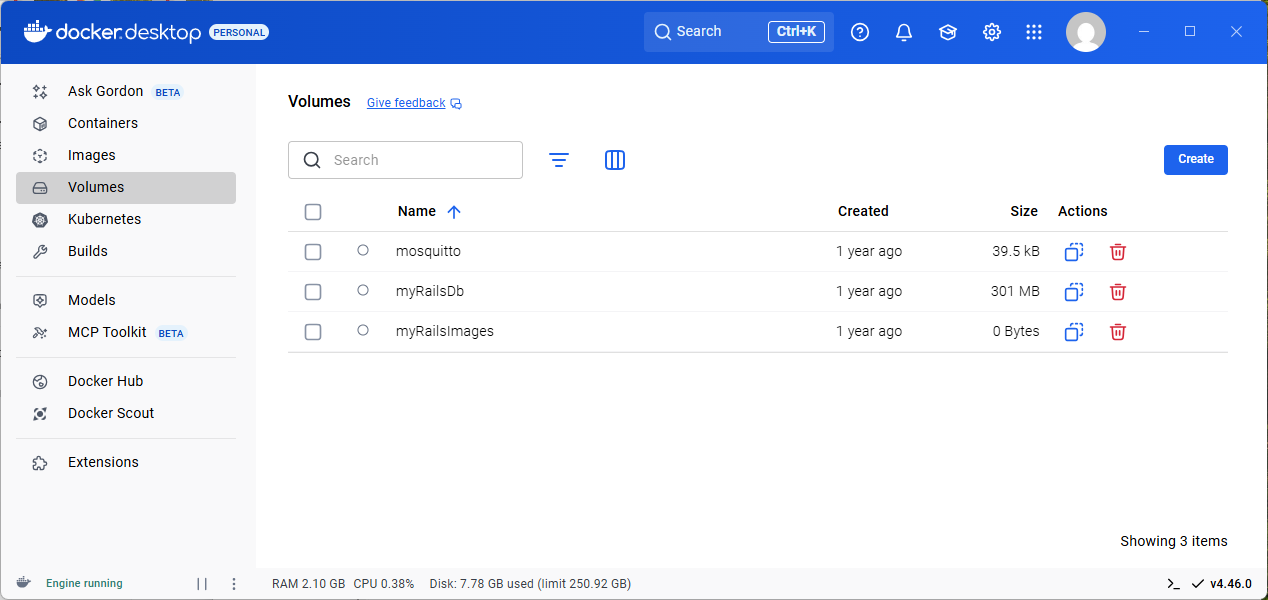
\includegraphics[scale=0.4]{../Images/volumes-ms.png}
    \caption{Docker Desktop Volumes}
    \label{fig:volumes-ms}
\end{figure}
\begin{figure}[H]
    \centering
    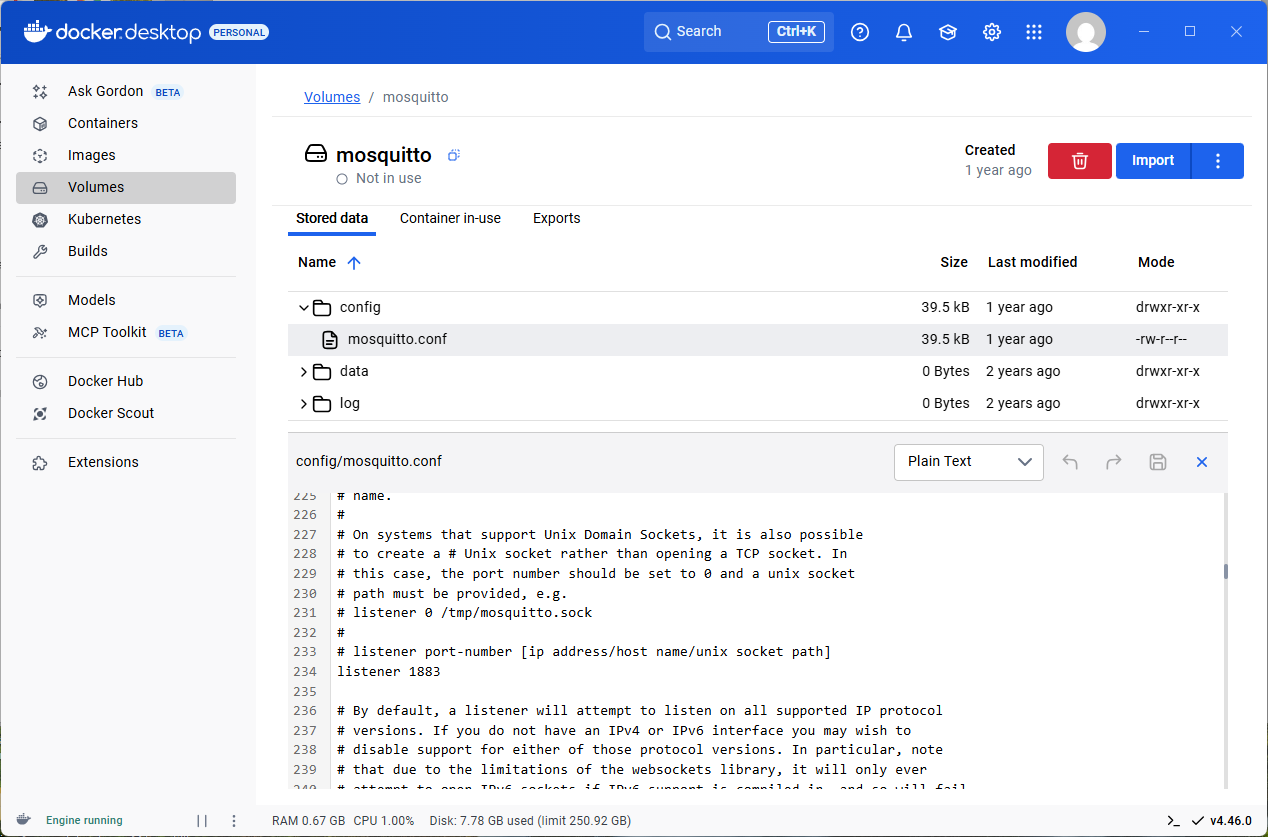
\includegraphics[scale=0.4]{../Images/edit-config-win.png}
    \caption{Mosquitto Configuration File}
    \label{fig:mosquitto-config}
\end{figure}
The following screenshots show the Docker commands used to create the Docker environment and run all of the \gls{rails} Docker containers.
\begin{figure}[H]
    \centering
    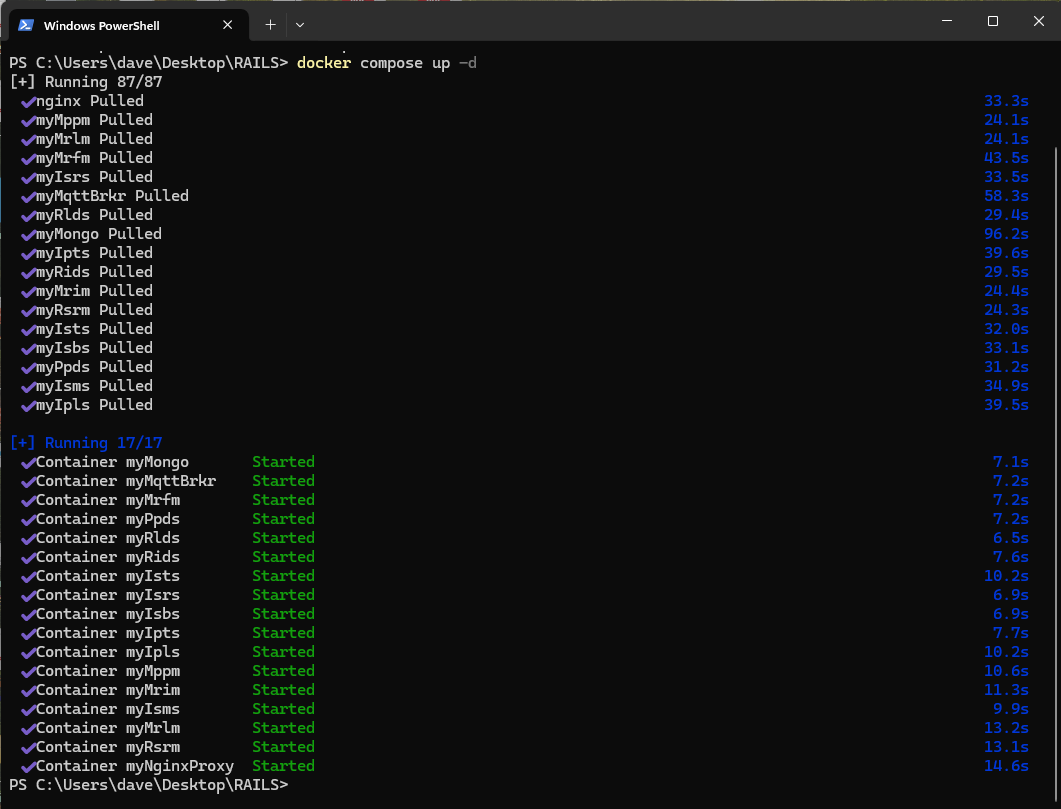
\includegraphics[scale=0.4]{../Images/dc-up-win.png}
    \caption{Windows Docker Compose Up}
    \label{fig:docker-compose-up} 
\end{figure}
The following screenshots confirm the Docker containers are running.
\begin{figure}[H]
    \centering
    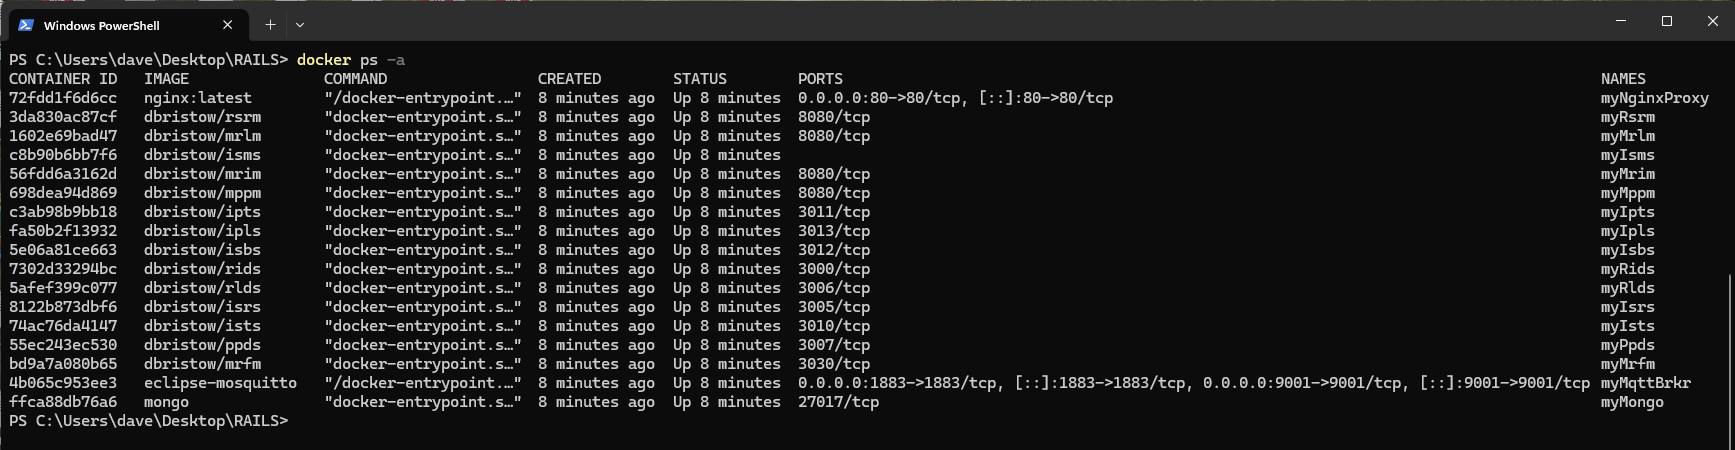
\includegraphics[scale=0.37]{../Images/ps-win.png}
    \caption{Windows Docker PS}
    \label{fig:docker-cmds-2}
\end{figure}
\begin{figure}[H]
    \centering
    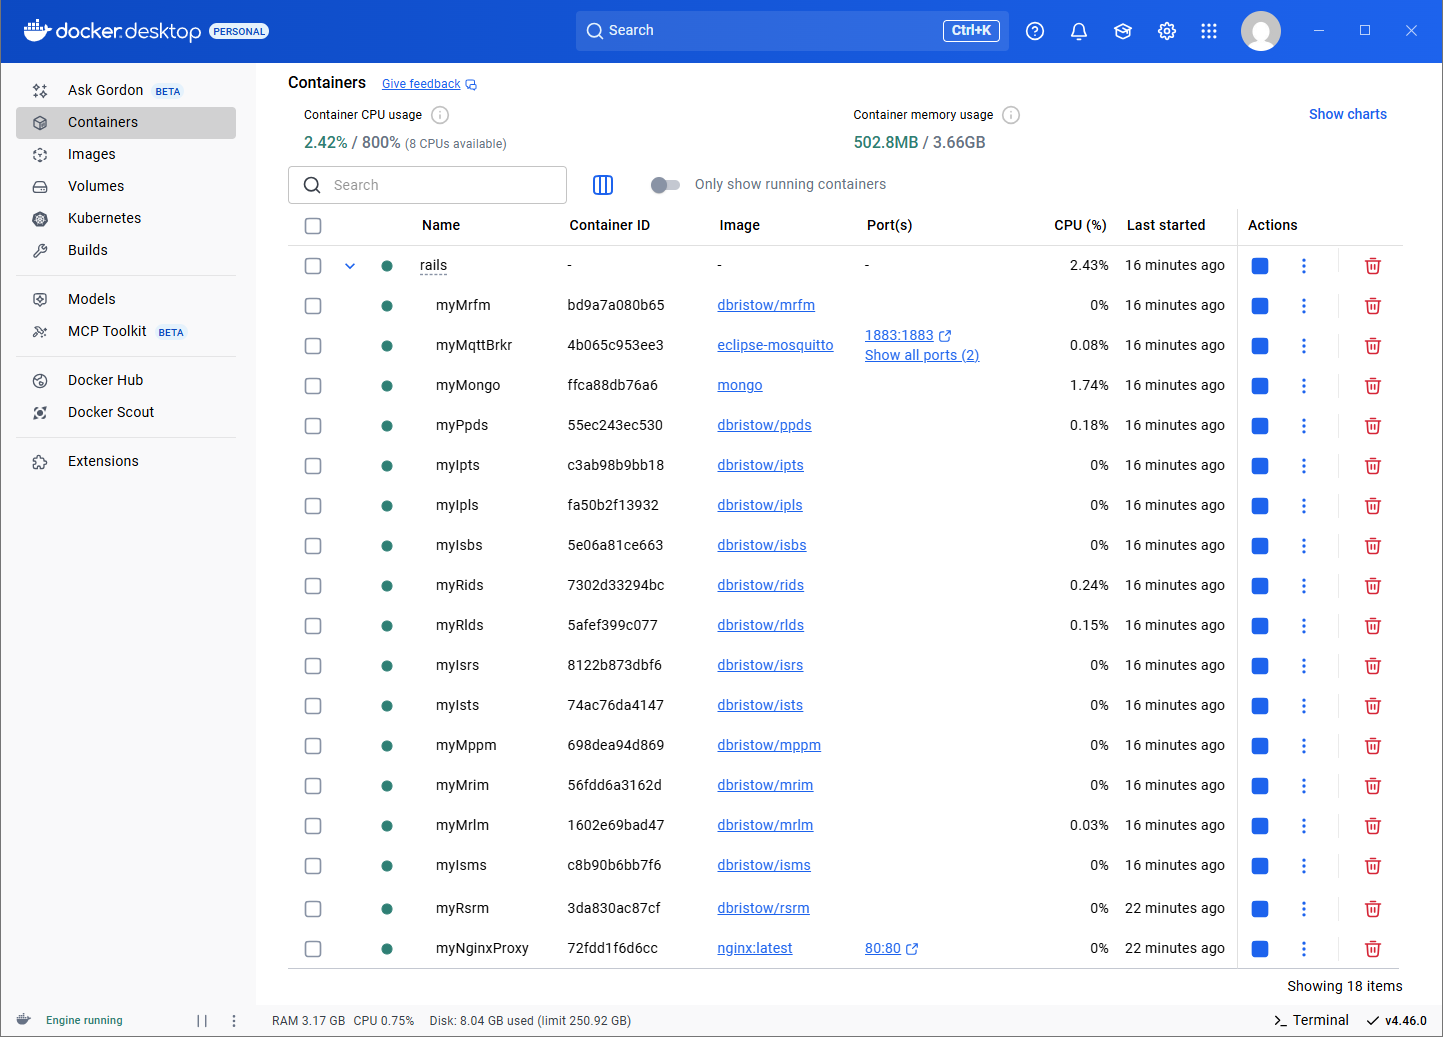
\includegraphics[scale=0.45]{../Images/docker-containers-win.png}
    \caption{Windows Docker Desktop Containers}
    \label{fig:docker-cmds-2}
\end{figure}
Once the Docker containers are running, the \gls{rails} \glspl{spa} can be accessed from a web browser (Chrome). The following screenshots show the \gls{rails} \glspl{spa} running in a web browser.
\begin{figure}[H]
    \centering
    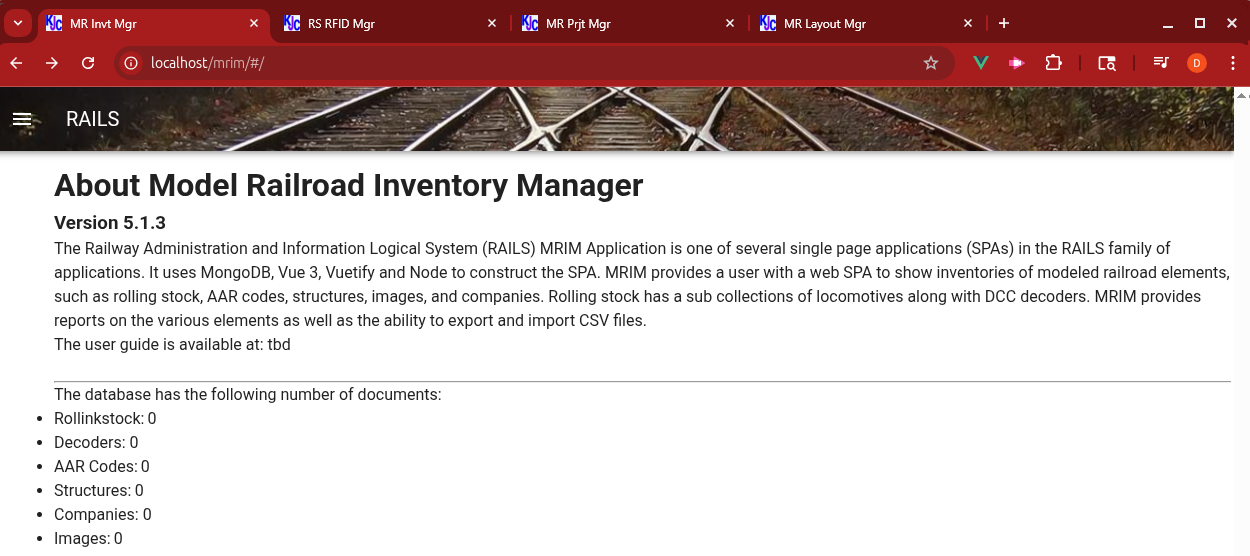
\includegraphics[scale=0.33]{../Images/mrim-home-0.png}
    \caption{RAILS MRIM Running}
    \label{fig:rails-mrim}
\end{figure}
\begin{figure}[H]
    \centering
    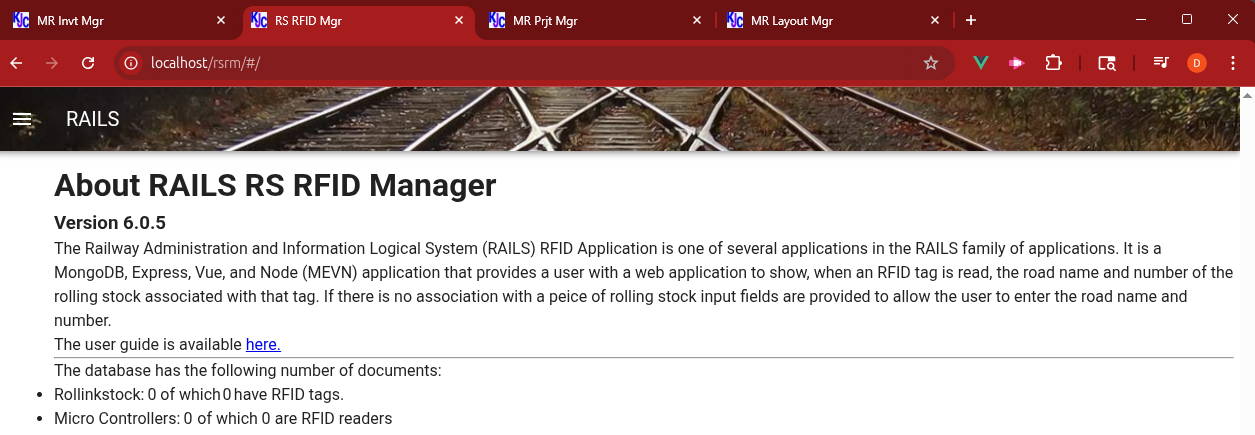
\includegraphics[scale=0.33]{../Images/rsrm-home.png}
    \caption{RAILS RSRM Running}
    \label{fig:rails-rsrm}
\end{figure}
\begin{figure}[H]
    \centering
    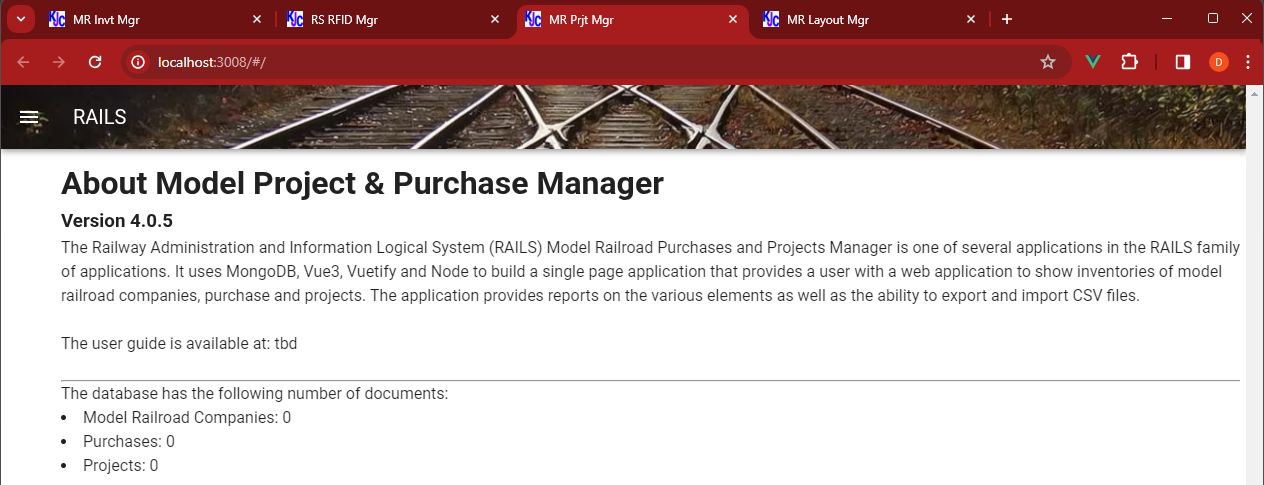
\includegraphics[scale=0.42]{../Images/mppm-home.png}
    \caption{RAILS MPPM Running}
    \label{fig:rails-mrim}
\end{figure}
\begin{figure}[H]
    \centering
    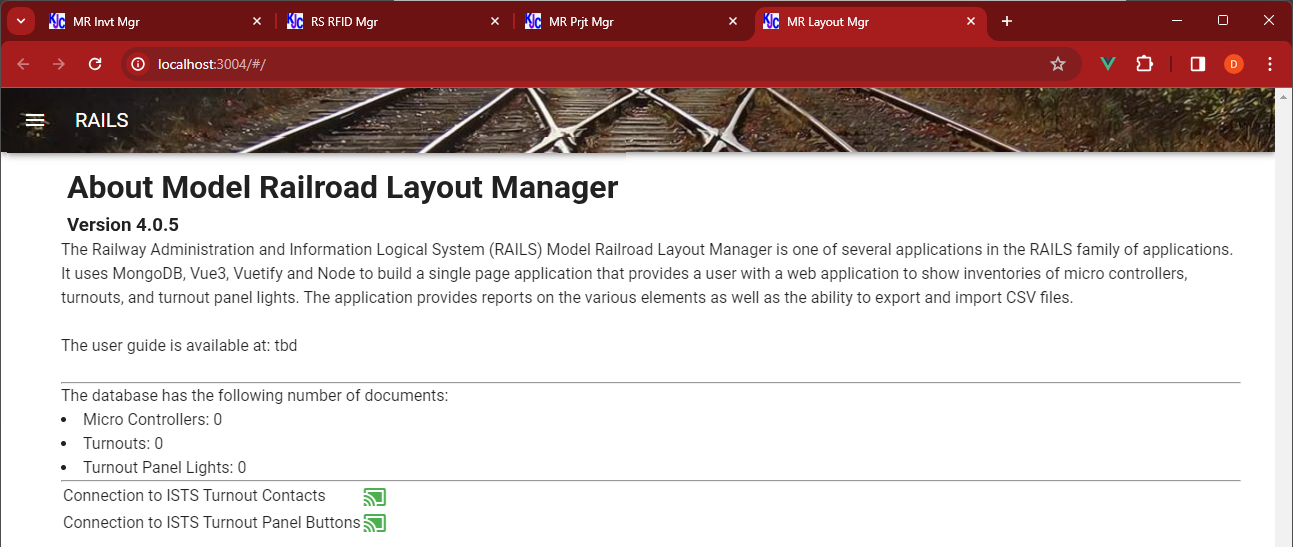
\includegraphics[scale=0.42]{../Images/mrlm-home.png}
    \caption{RAILS MRLM Running}
    \label{fig:rails-rsrm}
\end{figure}
The following screenshot shows the stopping and removal of the \gls{rails} Docker containers in a Windows environment.
\begin{figure}[H]
    \centering
    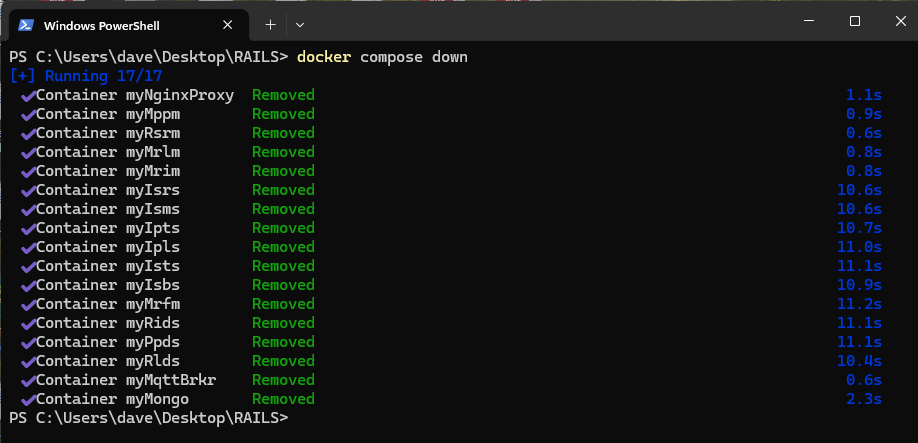
\includegraphics[scale=0.5]{../Images/dc-down-win.png}
    \caption{Windows Docker Compose Down}
    \label{fig:docker-cmds-3}
\end{figure}
\newpage
\section{Docker in a Linux Environment}
\label{sec:linux-cmds}
The following screenshot shows the initial Docker commands used to create the Docker environment in a Linux environment. The yellow highlighted text represents the edits of the mosquitto configuration file using the vi editor.
\begin{figure}[H]
    \centering
    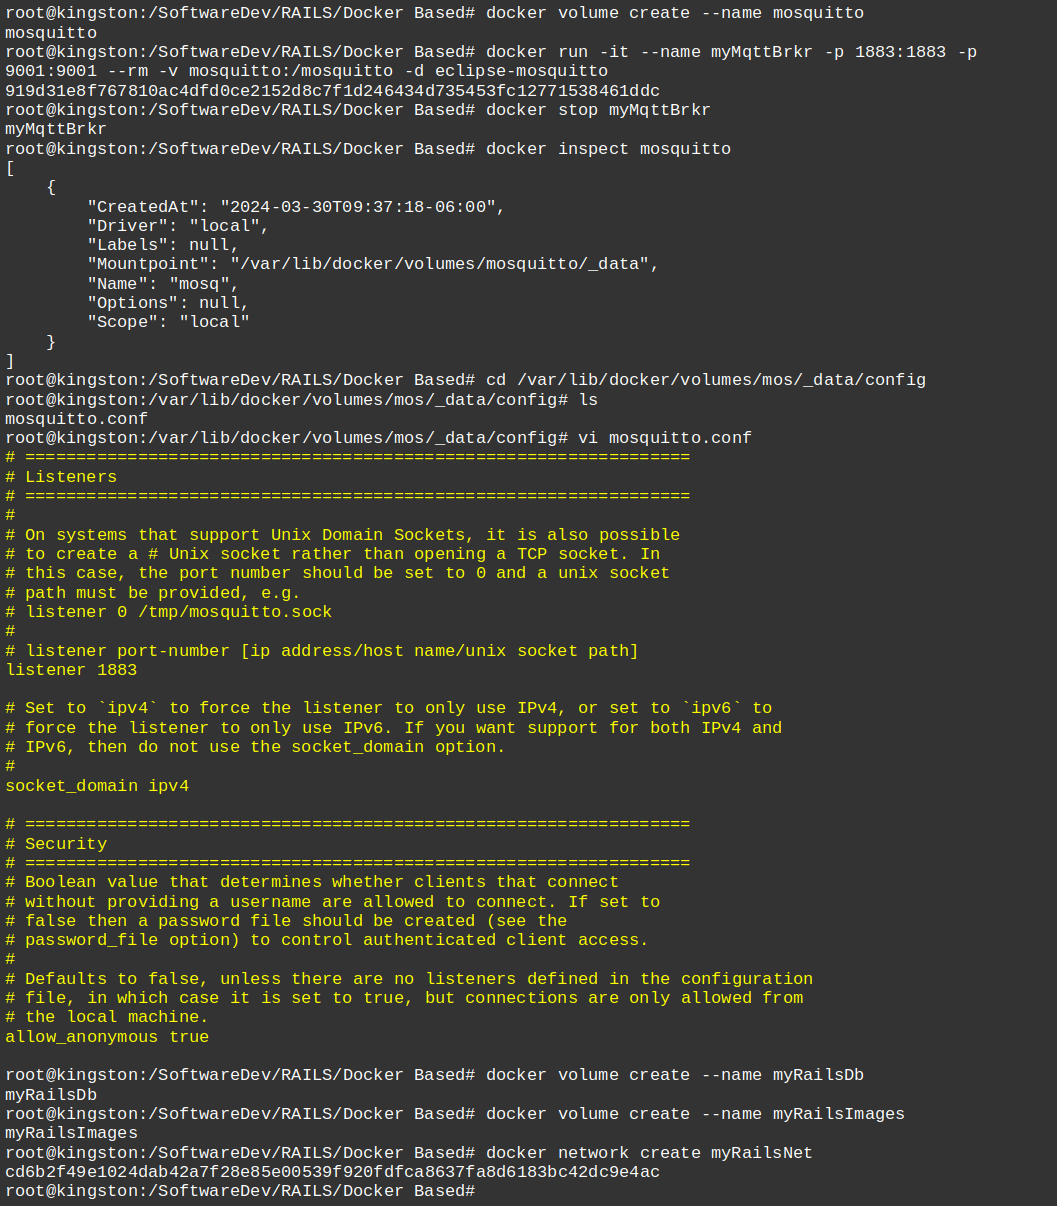
\includegraphics[scale=0.44]{../Images/mosquitto-edit-linux.png}
    \caption{Docker Setup mosquitto}
    \label{fig:linux-docker-cmds}
\end{figure}
The following screenshots show the Docker command used to pull images and run the \gls{rails} Docker containers in a Linux environment. The process starts by checking for images in the local repository, not finding any Docker will pull them from Docker Hub, the progress is displayed. Once all of the images are pulled, as seen in the top half of figure \ref{fig:linux-docker-cmds-2} Docker will then start each container. The bottom half of half of figure \ref{fig:linux-docker-cmds-2} shows the successful creation of all of the running containers.
\begin{figure}[H]
    \centering
    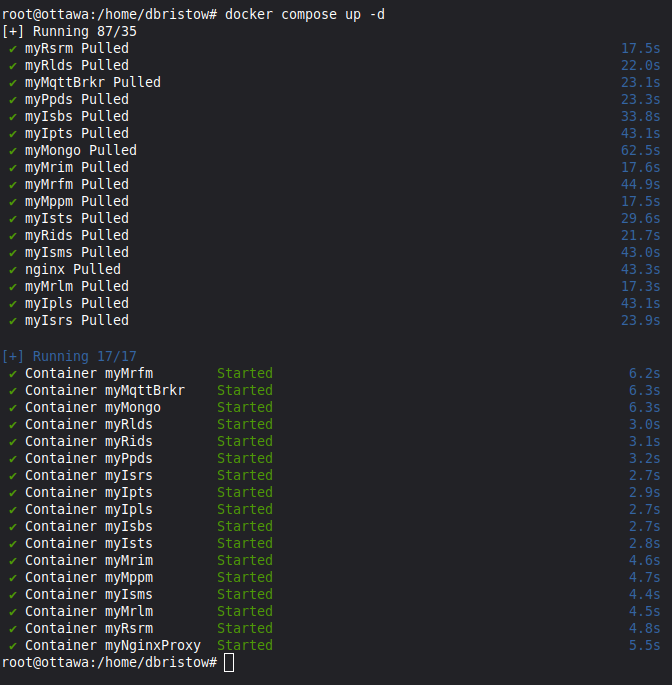
\includegraphics[scale=0.5]{../Images/docker-compose-up-linux.png}
    \caption{Linux Docker-Compose Up}
    \label{fig:linux-docker-cmds-2}
\end{figure}
The following screenshot shows a \gls{rails} \glspl{spa} running in a web browser (Chrome) in a Linux environment. The remaining \glspl{spa} can be accessed in the same manner.
\begin{figure}[H]
    \centering
    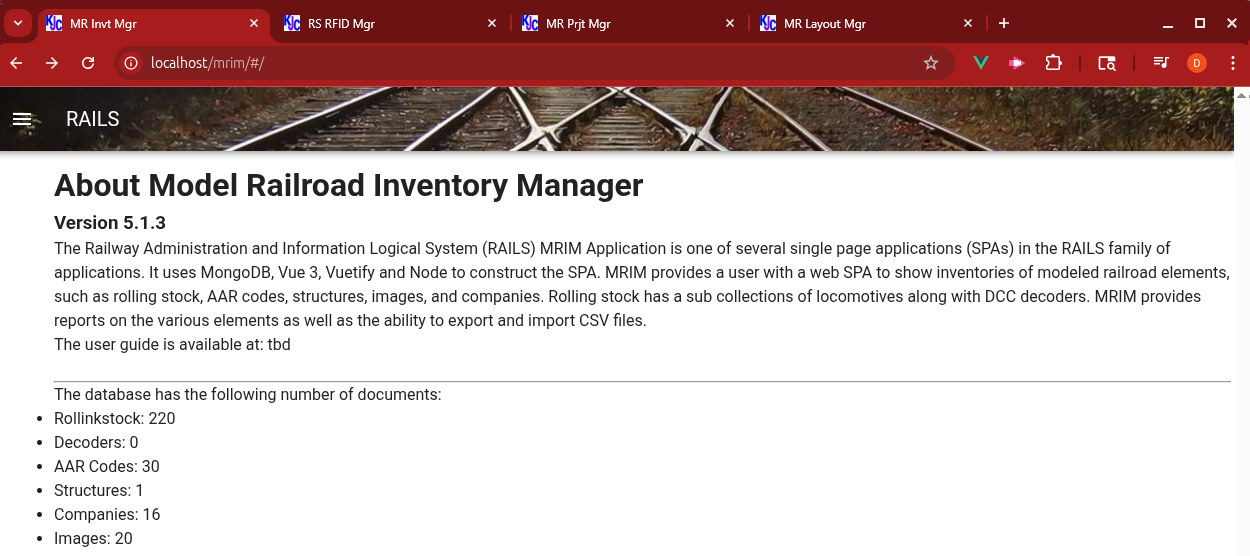
\includegraphics[scale=0.36]{../Images/mrim-home.png}
    \caption{RAILS MRIM Running}
    \label{fig:rails-mrim}
\end{figure}
The following screenshot shows the stopping and removal of the \gls{rails} Docker containers in a Linux environment.
\begin{figure}[H]
    \centering
    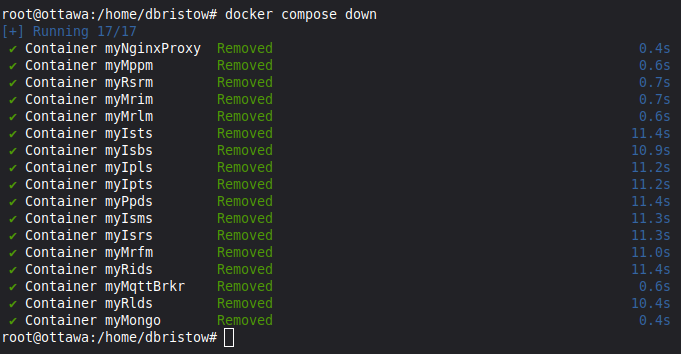
\includegraphics[scale=0.5]{../Images/docker-compose-down-linux.png}
    \caption{Linux Docker-Compose Down}
    \label{fig:linux-docker-cmds-4}
\end{figure}
\section{Docker in a MacOS Environment}
\label{sec:mac-cmds}
Docker itself doesn't run directly on MacOS 14 (Mojave). This is because Docker relies on a Linux kernel for containerization, and MacOS uses a different kernel. 
Similar to Windows there is a Docker Desktop software package that provides a complete Docker experience on MacOS. It includes:
\begin{itemize}
\item Docker Desktop installs and runs a lightweight Linux \gls{vm} in the background. This \gls{vm} typically uses LinuxKit, a minimal Linux distribution optimized for running Docker.
\item The Docker engine runs within the Linux \gls{vm}. This engine is responsible for managing Docker images, containers, and networks.
\item Docker Desktop provides a \gls{cli} for interacting with the Docker engine running in the VM. You can use familiar Docker commands to build, run, and manage containers.
\item Docker Desktop offers an optional GUI that allows you to manage containers visually.
\end{itemize}
The following screenshot shows the initial Docker commands used to create the Docker environment in a MacOS environment. Like Windows it is simpler to use Docker Desktop \gls{gui} to locate and edit the mosquitto configuration file.
Using the Docker Desktop to create the volumes and to edit the mosquitto configuration file, similarly to that done in Linux the result is shown in figure \ref{fig:mac-docker-volumes}
\begin{figure}[H]
    \centering
    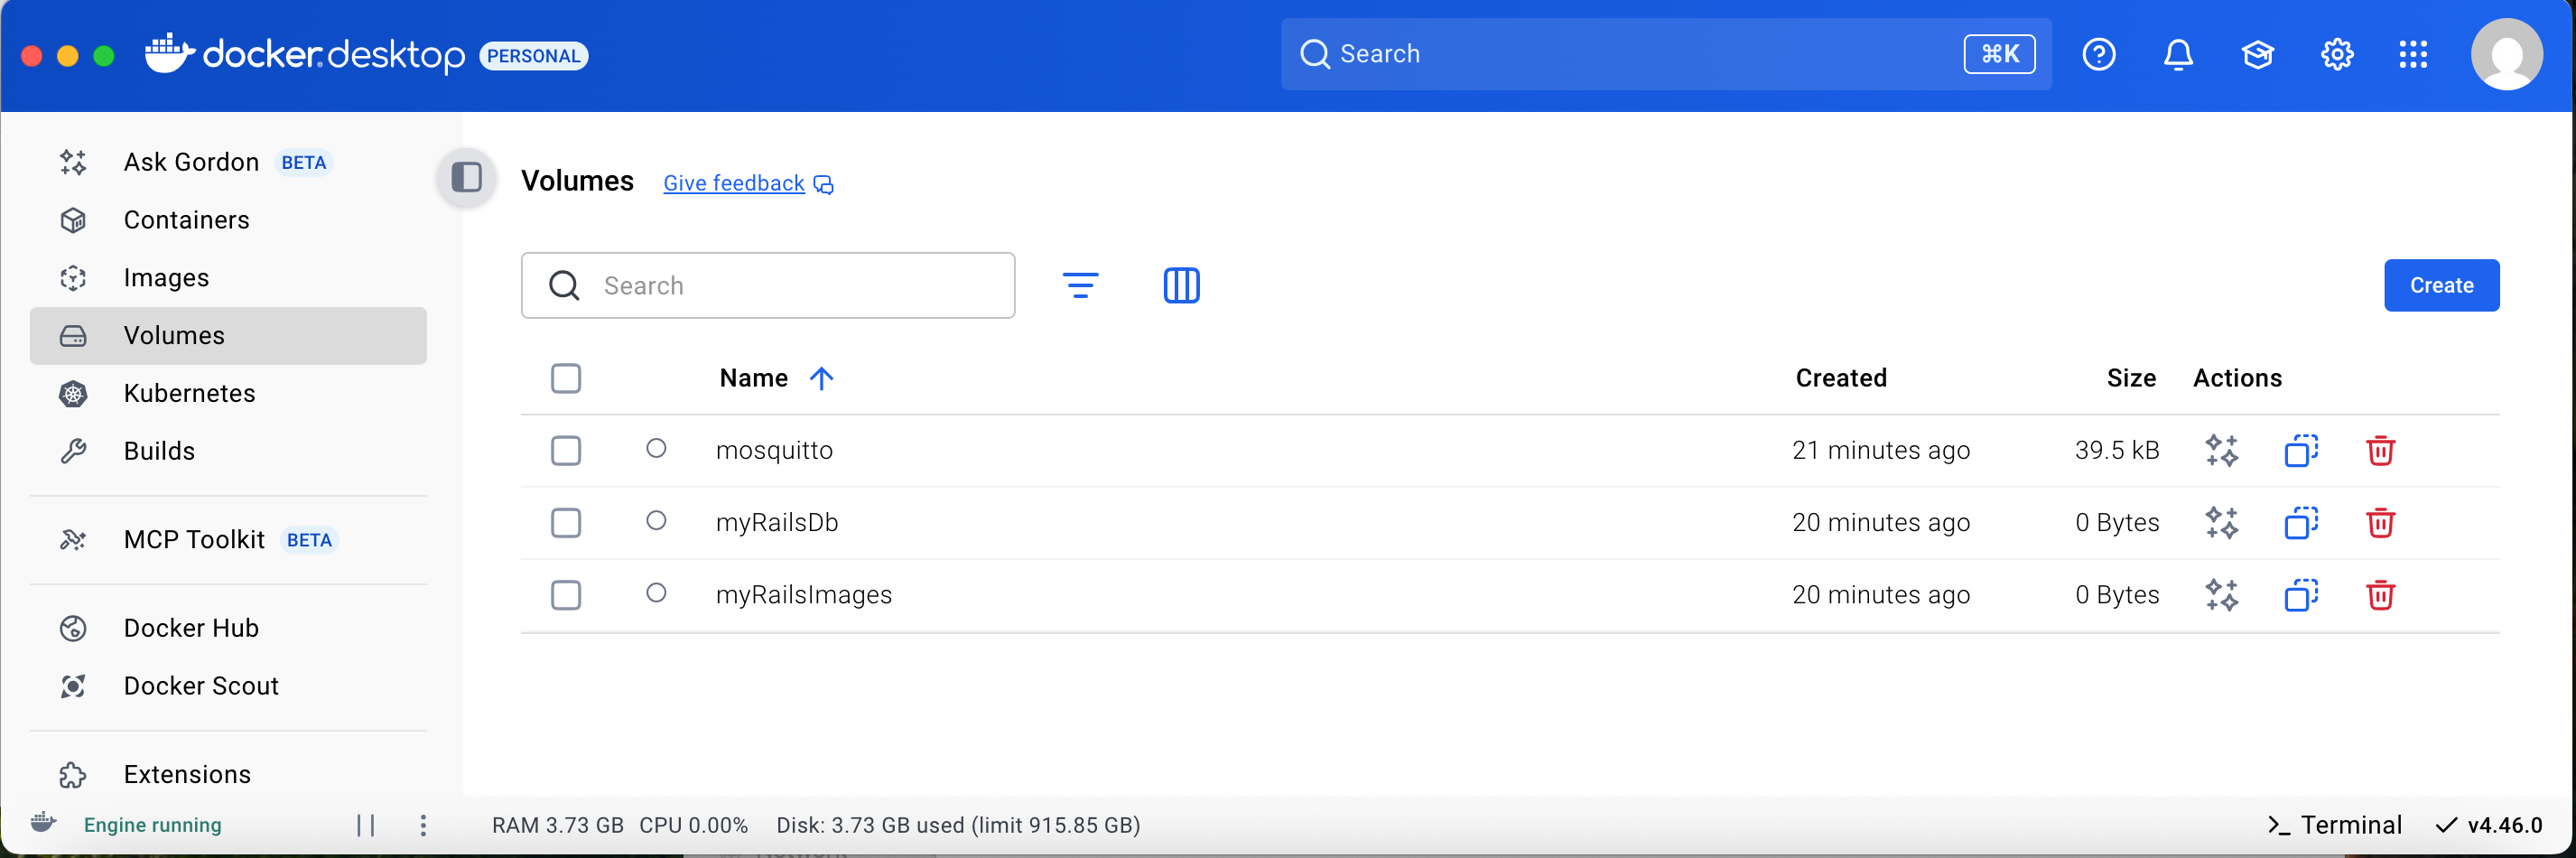
\includegraphics[scale=0.33]{../Images/volumes-mac.png}
    \caption{Mac Docker Desktop Volumes}
    \label{fig:mac-docker-volumes}
\end{figure}
Open a Mac terminal to initiate Docker Compose to setup and run the \gls{rails} container. Figure \ref{fig:mac-docker-compose-up1} is a snapshot showing the pulling of the images from Docker Hub. Figure \ref{fig:mac-docker-compose-up2} captures the process of pulling all of the images nearing completion. Figure \ref{fig:mac-docker-compose-up3} shows the terminal once the ``docker compose up -d'' command has completed and all of teh containers are running.
\begin{figure}[H]
    \centering
    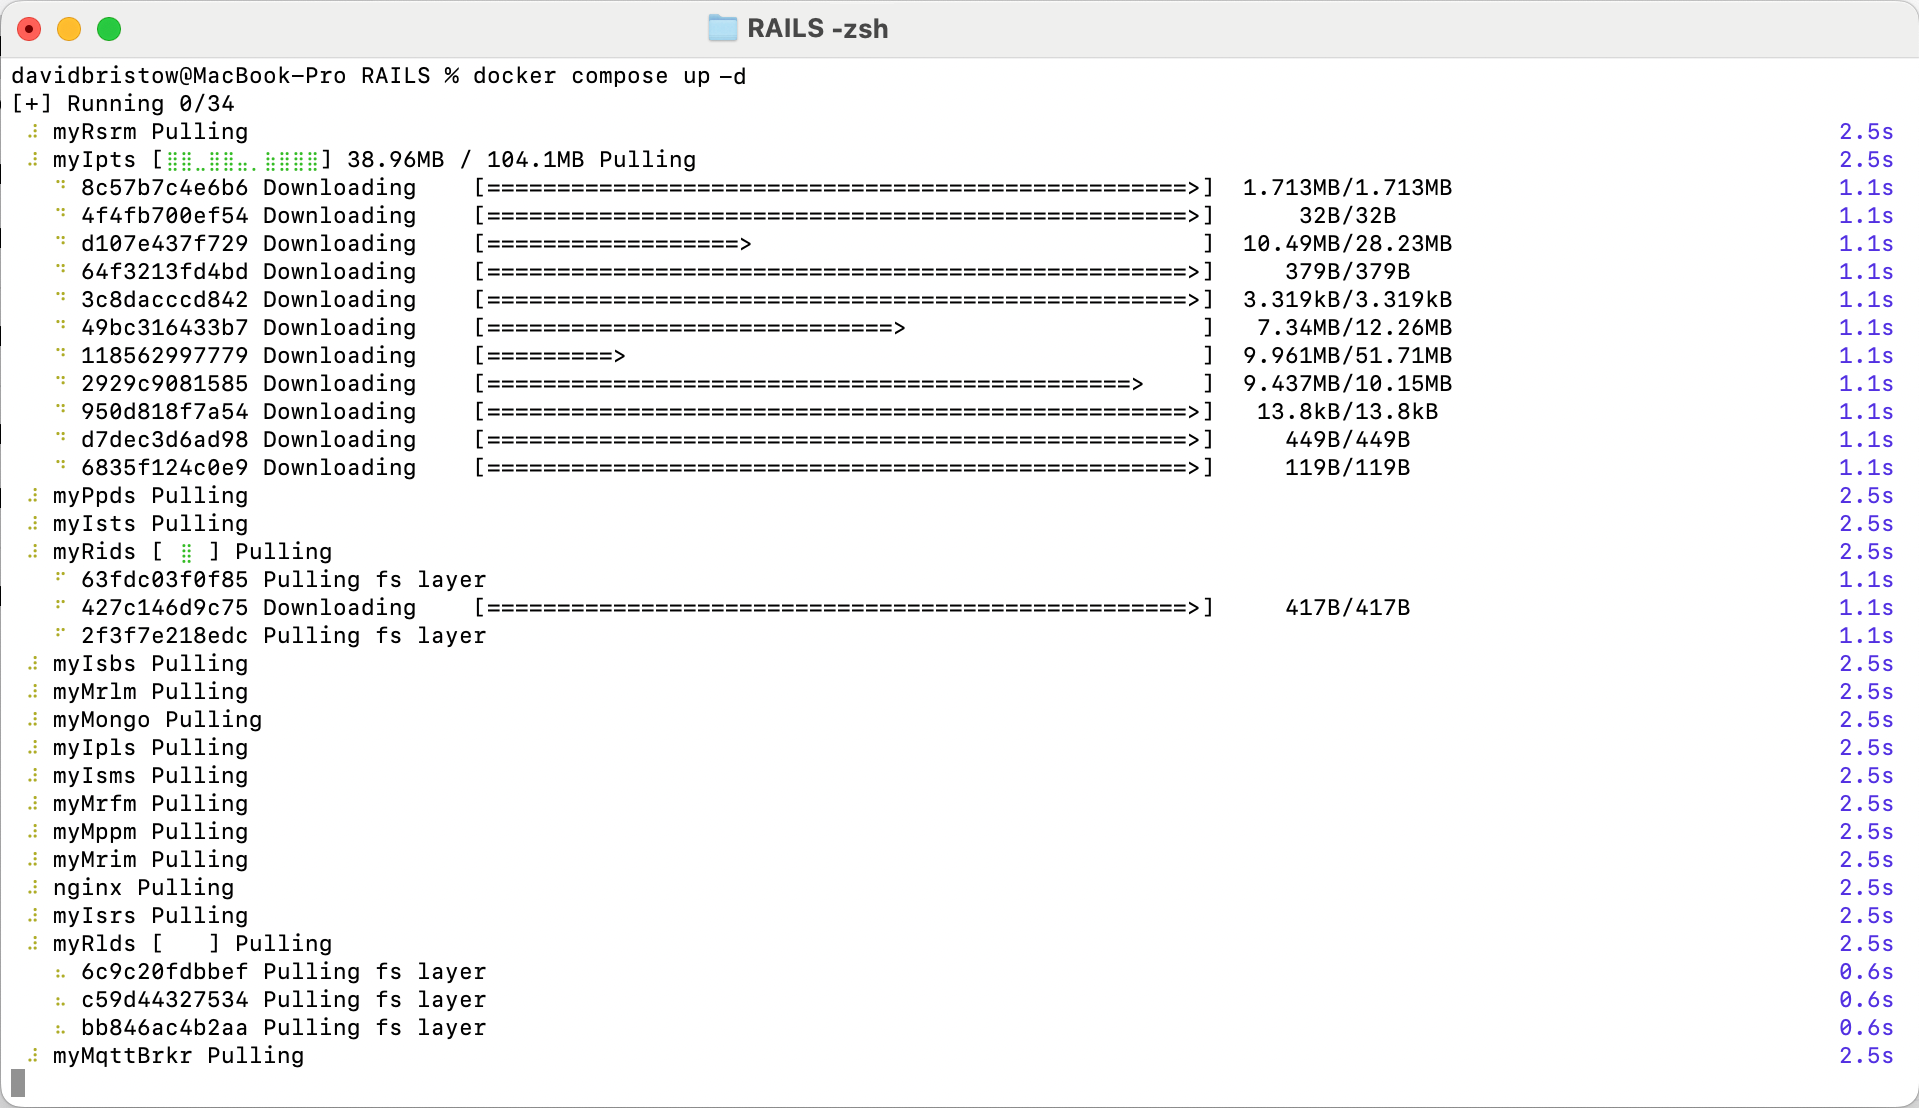
\includegraphics[scale=0.4]{../Images/dc-up-progress1-mac.png}
    \caption{MacOS Docker Compose Up Pulls}
    \label{fig:mac-docker-compose-up1}
\end{figure}
\begin{figure}[H]
    \centering
    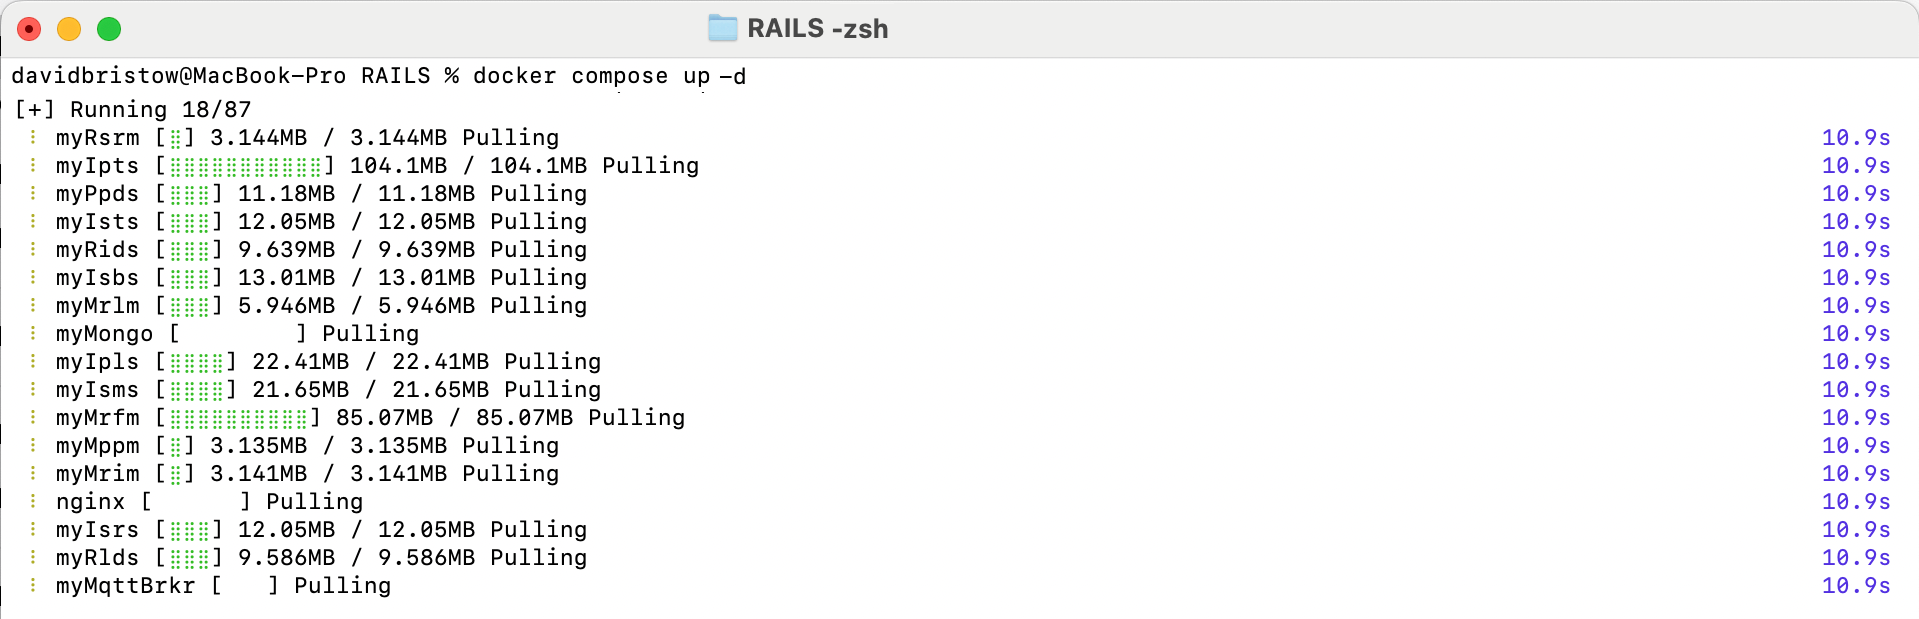
\includegraphics[scale=0.4]{../Images/dc-up-progress2-mac.png}
    \caption{MacOS Docker Compose Up Completing Pulls}
    \label{fig:mac-docker-compose-up2}
\end{figure}
\begin{figure}[H]
    \centering
    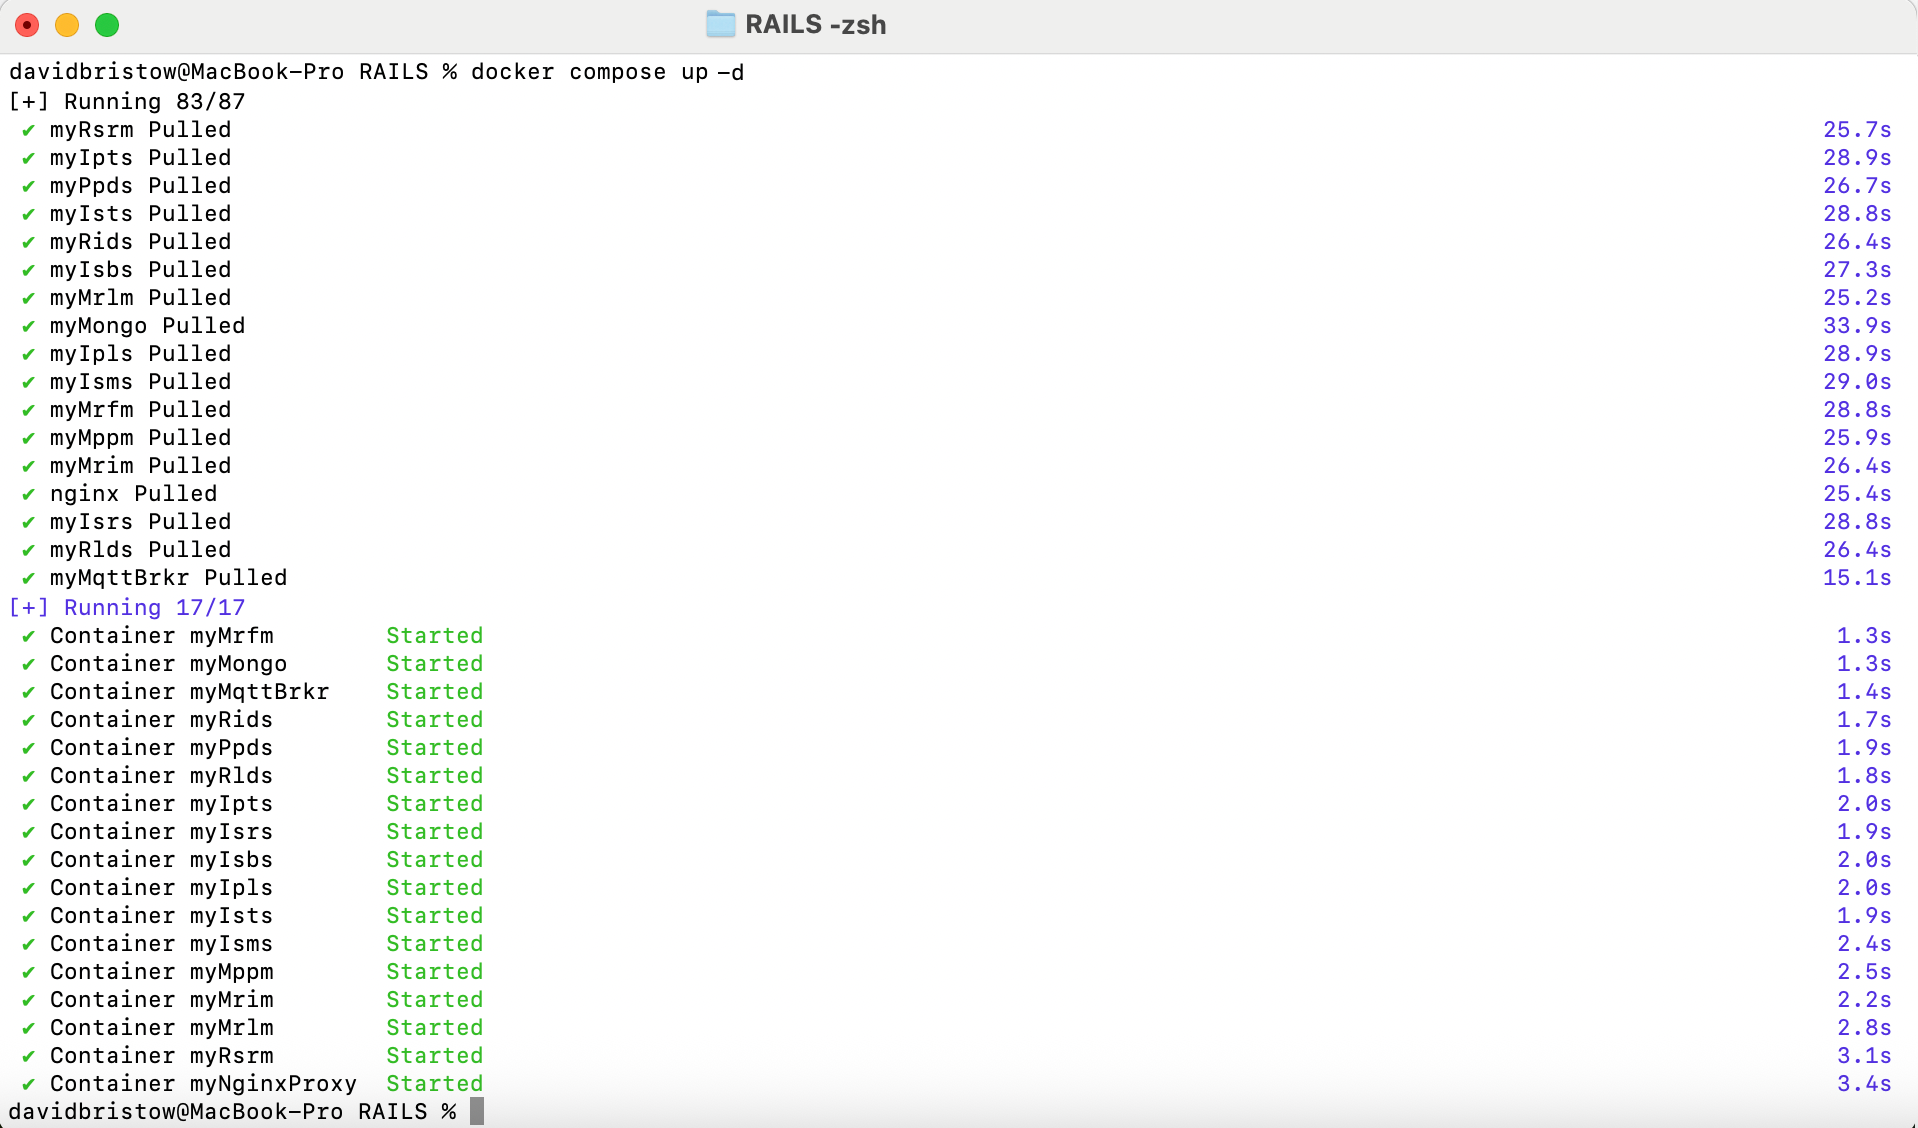
\includegraphics[scale=0.4]{../Images/dc-up-progress3-mac.png}
    \caption{MacOS Docker Compose Up Started}
    \label{fig:mac-docker-compose-up3}
\end{figure}
Figure \ref{fig:mac-docker-desktop-images} shows in the Docker Desktop \gls{gui} that all the images are now local to the Mac.
\begin{figure}[H]
    \centering
    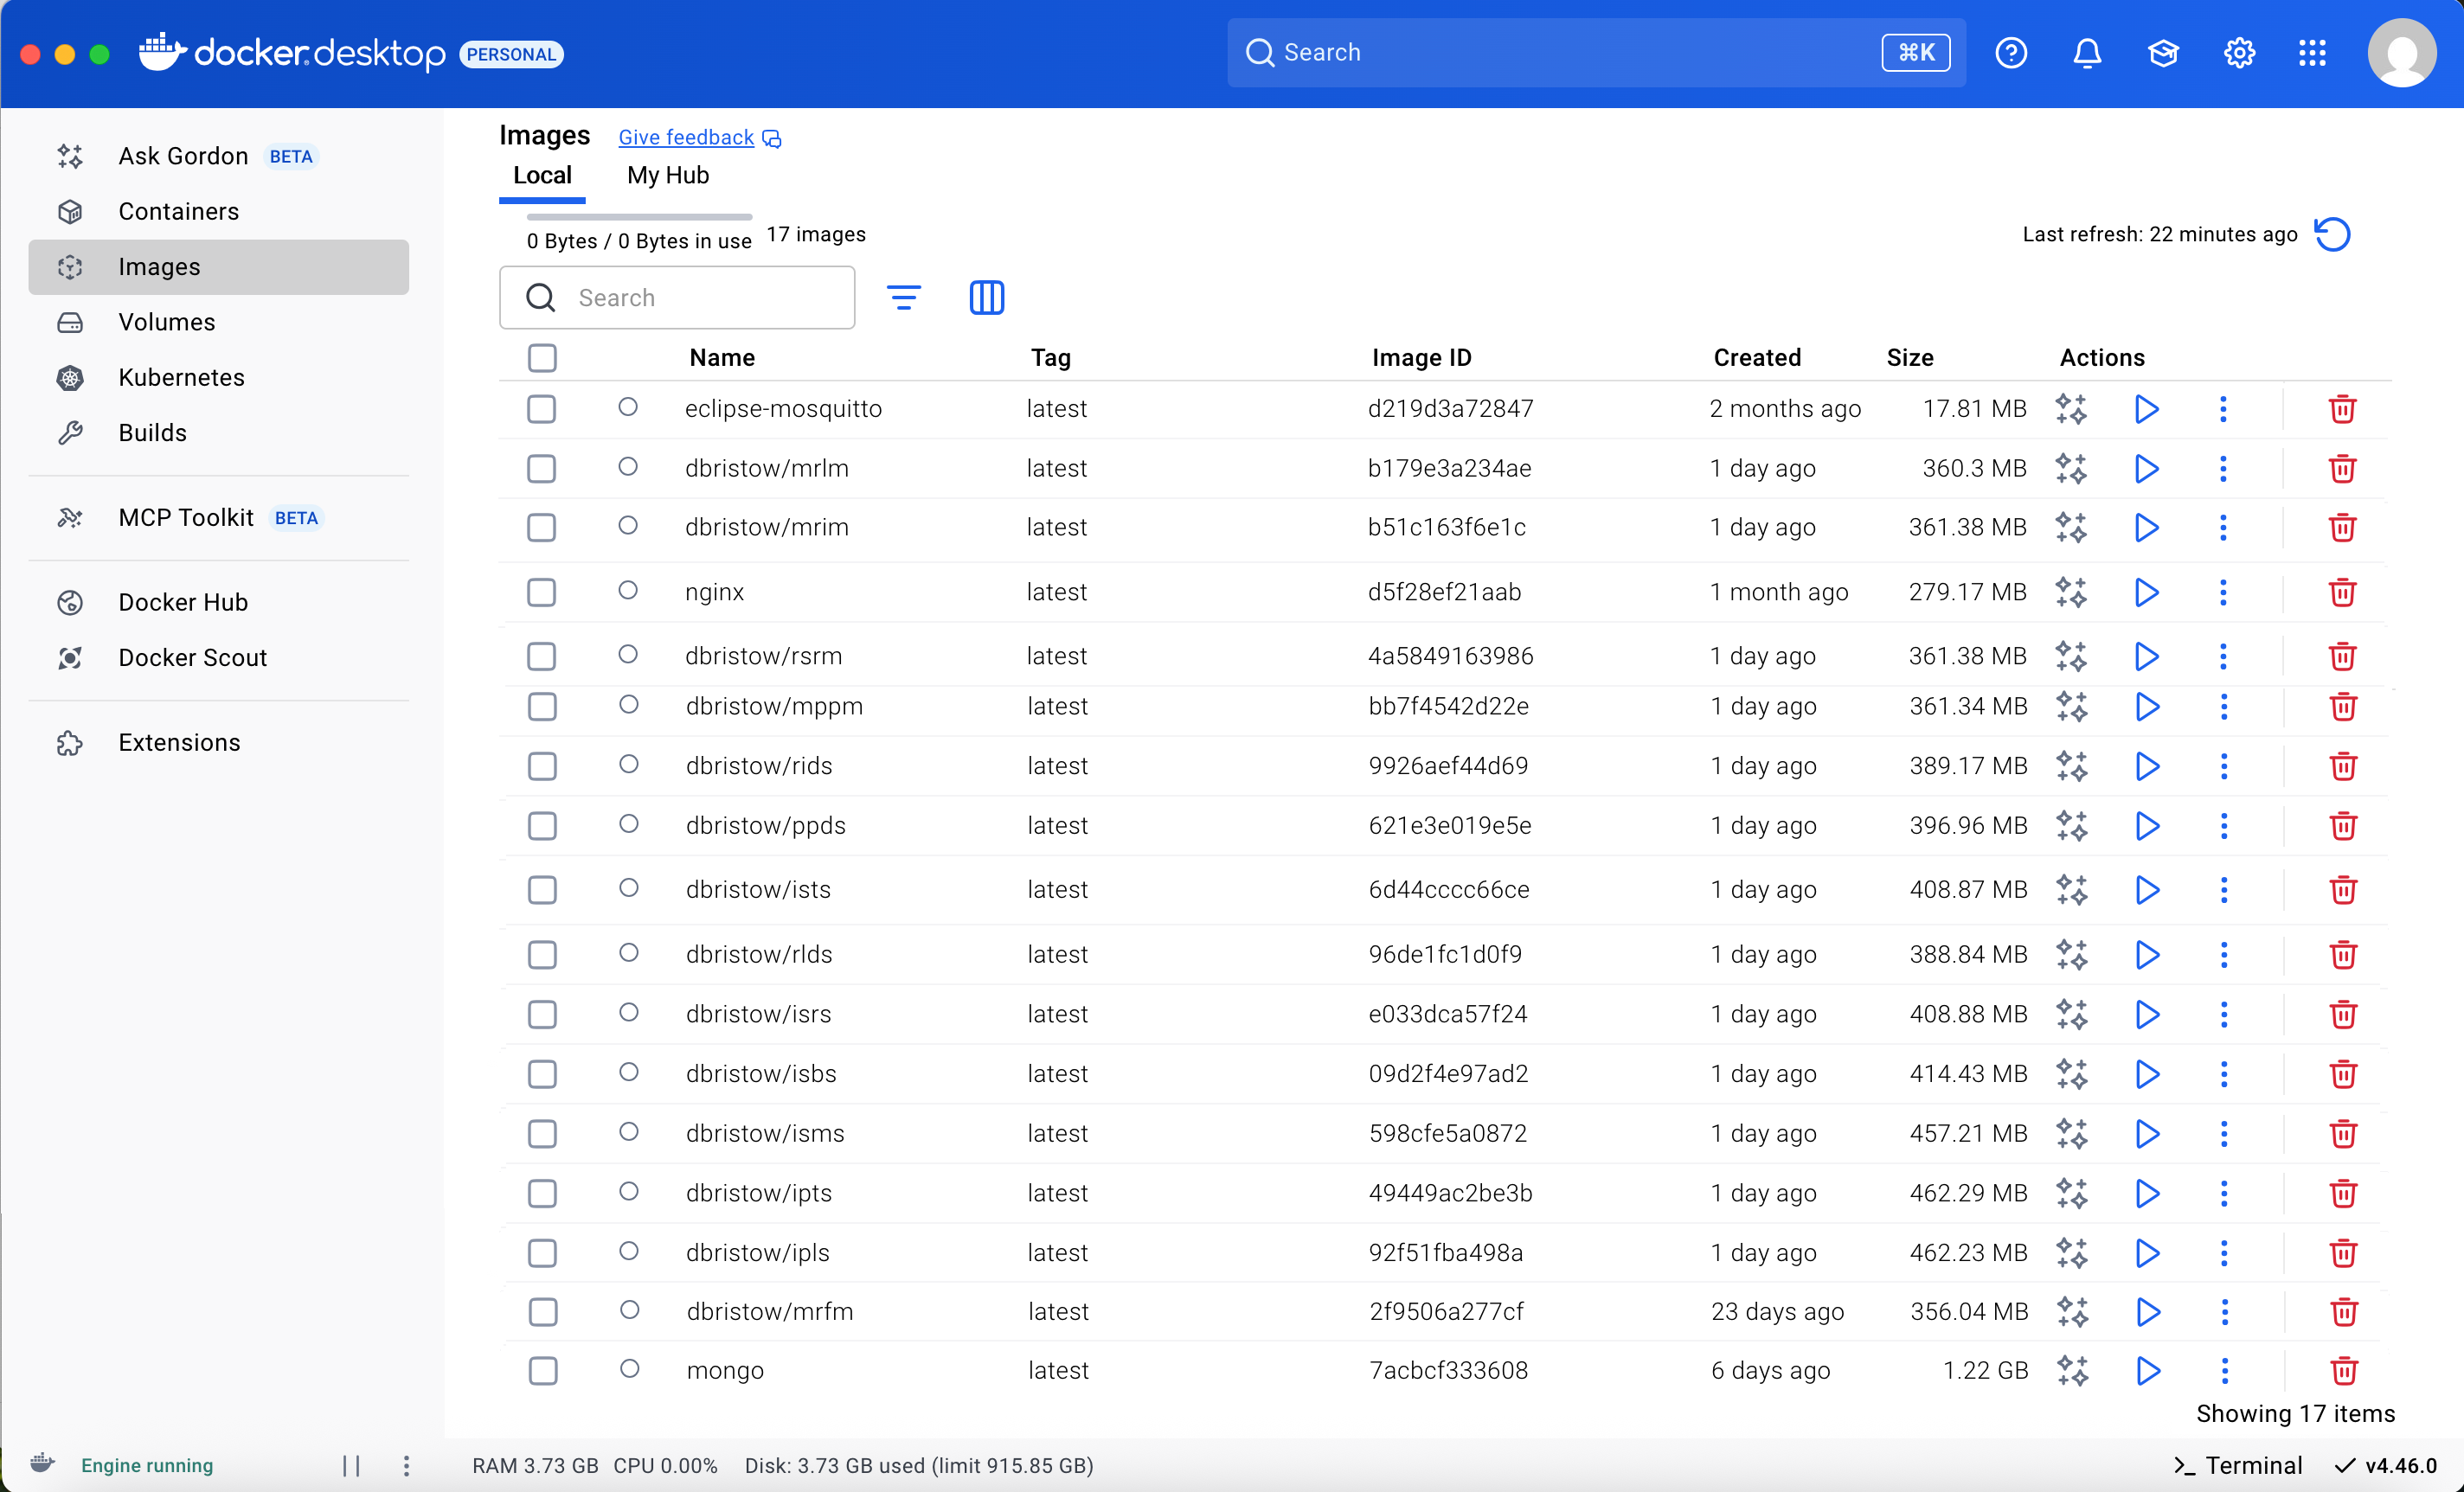
\includegraphics[scale=0.3]{../Images/images-mac.png}
    \caption{MacOS Docker Desktop Images}
    \label{fig:mac-docker-desktop-images}
\end{figure}
The following screenshot shows a \gls{rails} \glspl{spa} running in a web browser (Safari) in a MacOS environment. The remaining \glspl{spa} can be accessed in the same manner.
\begin{figure}[H]
    \centering
    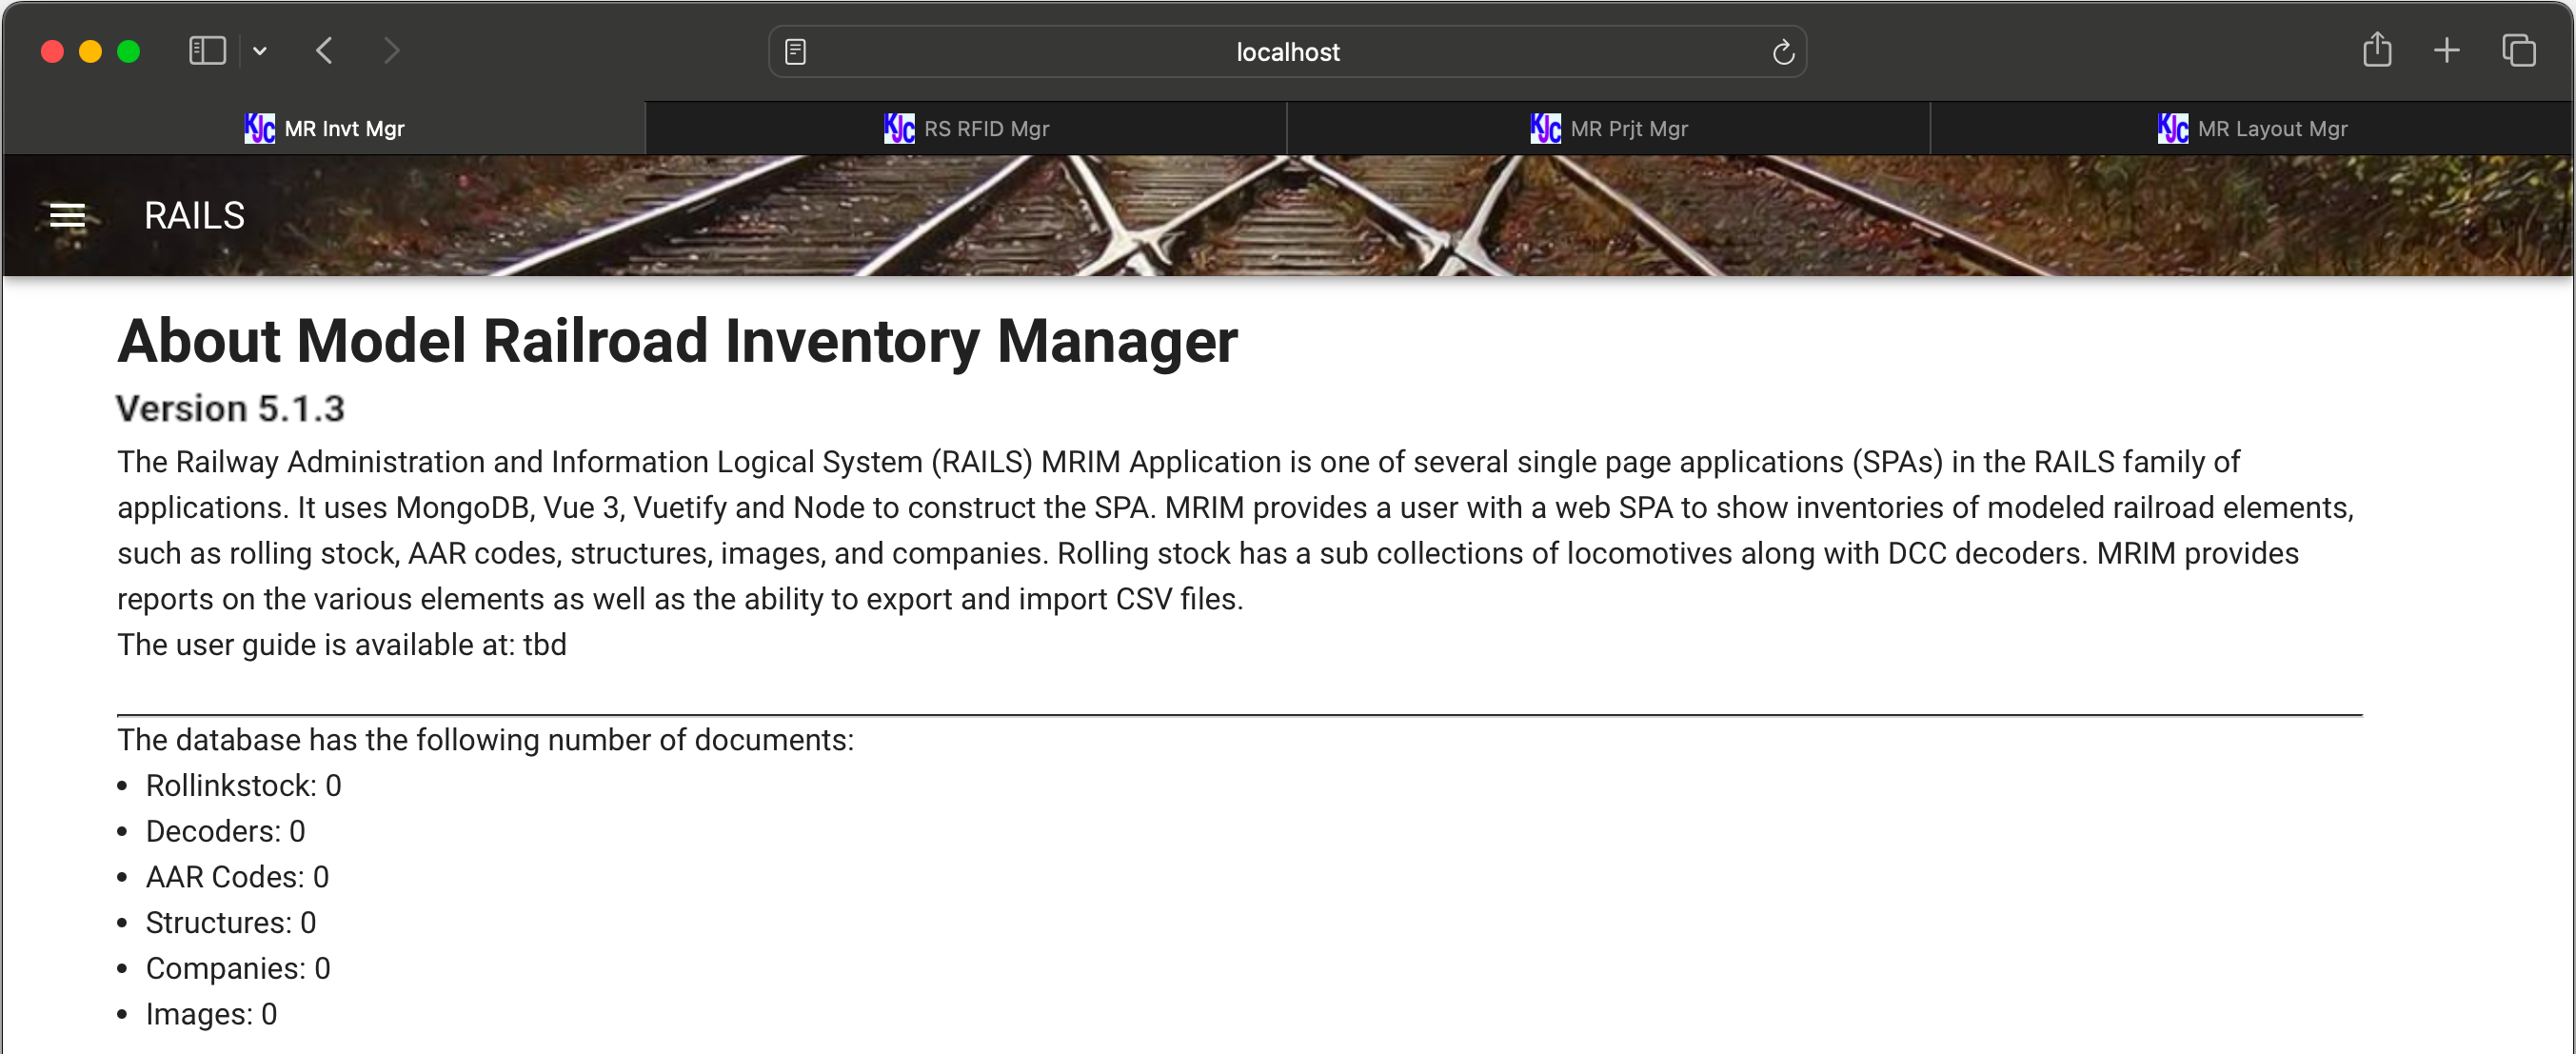
\includegraphics[scale=0.3]{../Images/mrim-home-mac.png}
    \caption{RAILS MRIM Running}
    \label{fig:rails-mrim}
\end{figure}
The following screenshot shows the stopping and removal of the \gls{rails} Docker containers in a MacOS environment.
\begin{figure}[H]
    \centering
    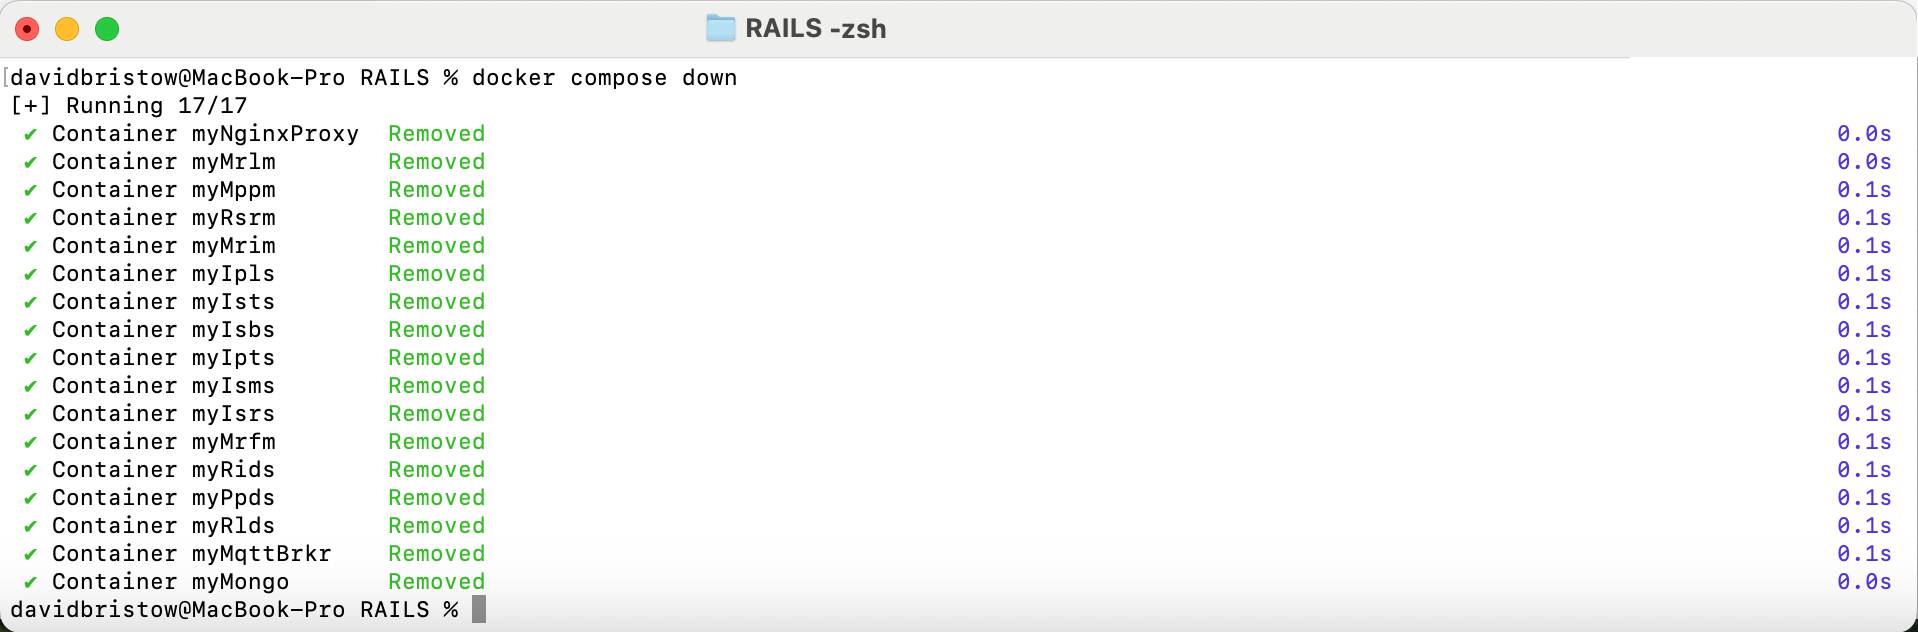
\includegraphics[scale=0.45]{../Images/dc-down-mac.png}
    \caption{MacOS DockerCompose Down}
    \label{fig:mac-docker-cmds-3}
\end{figure}
